\documentclass[bachelor, och, labwork]{shiza}
% параметр - тип обучения - одно из значений:
%    spec     - специальность
%    bachelor - бакалавриат (по умолчанию)
%    master   - магистратура
% параметр - форма обучения - одно из значений:
%    och   - очное (по умолчанию)
%    zaoch - заочное
% параметр - тип работы - одно из значений:
%    referat    - реферат
%    coursework - курсовая работа (по умолчанию)
%    diploma    - дипломная работа
%    pract      - отчет по практике
% параметр - включение шрифта
%    times    - включение шрифта Times New Roman (если установлен)
%               по умолчанию выключен
\usepackage{subfigure}
\usepackage{tikz,pgfplots}
\pgfplotsset{compat=1.5}
\usepackage{float}

%\usepackage{titlesec}
\setcounter{secnumdepth}{4}
%\titleformat{\paragraph}
%{\normalfont\normalsize}{\theparagraph}{1em}{}
%\titlespacing*{\paragraph}
%{35.5pt}{3.25ex plus 1ex minus .2ex}{1.5ex plus .2ex}

\titleformat{\paragraph}[block]
{\hspace{1.25cm}\normalfont}
{\theparagraph}{1ex}{}
\titlespacing{\paragraph}
{0cm}{2ex plus 1ex minus .2ex}{.4ex plus.2ex}

% --------------------------------------------------------------------------%


\usepackage[T2A]{fontenc}
\usepackage[utf8]{inputenc}
\usepackage{graphicx}
\graphicspath{ {./images/} }
\usepackage{tempora}

\usepackage[sort,compress]{cite}
\usepackage{amsmath}
\usepackage{amssymb}
\usepackage{amsthm}
\usepackage{fancyvrb}
\usepackage{listings}
\usepackage{listingsutf8}
\usepackage{longtable}
\usepackage{array}
\usepackage[english,russian]{babel}

\usepackage[colorlinks=false]{hyperref}
\usepackage{url}

\usepackage{underscore}
\usepackage{setspace}
\usepackage{indentfirst} 
\usepackage{mathtools}
\usepackage{amsfonts}
\usepackage{enumitem}
\usepackage{tikz}
\usepackage{minted}

\newcommand{\eqdef}{\stackrel {\rm def}{=}}
\newcommand{\specialcell}[2][c]{%
\begin{tabular}[#1]{@{}c@{}}#2\end{tabular}}

\renewcommand\theFancyVerbLine{\small\arabic{FancyVerbLine}}

\newtheorem{lem}{Лемма}

\begin{document}

% Кафедра (в родительном падеже)
\chair{теоретических основ компьютерной безопасности и криптографии}

% Тема работы
\title{Факторизация целых чисел}

% Курс
\course{5}

% Группа
\group{531}

% Факультет (в родительном падеже) (по умолчанию "факультета КНиИТ")
\department{факультета КНиИТ}

% Специальность/направление код - наименование
%\napravlenie{09.03.04 "--- Программная инженерия}
%\napravlenie{010500 "--- Математическое обеспечение и администрирование информационных систем}
%\napravlenie{230100 "--- Информатика и вычислительная техника}
%\napravlenie{231000 "--- Программная инженерия}
\napravlenie{100501 "--- Компьютерная безопасность}

% Для студентки. Для работы студента следующая команда не нужна.
% \studenttitle{Студентки}

% Фамилия, имя, отчество в родительном падеже
\author{Улитина Ивана Владимировича}

% Заведующий кафедрой
% \chtitle{} % степень, звание
% \chname{}

%Научный руководитель (для реферата преподаватель проверяющий работу)
\satitle{профессор} %должность, степень, звание
\saname{В. А. Молчанов}

% Руководитель практики от организации (только для практики,
% для остальных типов работ не используется)
% \patitle{к.ф.-м.н.}
% \paname{С.~В.~Миронов}

% Семестр (только для практики, для остальных
% типов работ не используется)
%\term{8}

% Наименование практики (только для практики, для остальных
% типов работ не используется)
%\practtype{преддипломная}

% Продолжительность практики (количество недель) (только для практики,
% для остальных типов работ не используется)
%\duration{4}

% Даты начала и окончания практики (только для практики, для остальных
% типов работ не используется)
%\practStart{30.04.2019}
%\practFinish{27.05.2019}

% Год выполнения отчета
\date{2023}

\maketitle

% Включение нумерации рисунков, формул и таблиц по разделам
% (по умолчанию - нумерация сквозная)
% (допускается оба вида нумерации)
% \secNumbering

%-------------------------------------------------------------------------------------------

\section{Постановка задачи}

    \textbf{Цель работы} - изучение основных методов факторизации целых чисел и
    их программная реализация. 

    Порядок выполнения работы:
    \begin{enumerate}
        \item Рассмотреть $\rho$-метод Полларда разложения целых чисел на
        множители и привести его программную реализацию;
        \item Рассмотреть $(\rho - 1)$-метод Полларда разложения целых чисел на
        множители и привести его программную реализацию;
        \item Рассмотреть метод цепных дробей разложения целых чисел на
        множители и привести его программную реализацию;
    \end{enumerate}

\section{Теоретические сведения}

    \subsection{$\rho$-метод Полларда}

        Это вероятностный алгоритм факторизации целых чисел, с помощью которого
        разложено число $F_8 = 2^{2^8} + 1$.

        С помощью случайного сжимающего отображения $f: Z_n \to Z_n$ (например,
        многочлена) строится рекуррентная последовательность $x_{i + 1} = f(x_i)
        \pmod n$ со случайным начальным условием $x_0 \in Z_n$ и проверяется $$1
        < \text{НОД}(x_i - x_k, n) < n.$$

        Так как составное число $n$ имеет простой делитель $p < \sqrt{n}$, то
        последовательность $\{x_i\}$ имеет период $\leq n$ и последовательность
        $\{x_i \pmod p\}$ имеет период $\leq p$. Значит, с большой вероятностью
        найдутся такие значения последовательности $x_i, x_k$, для которых $$x_i
        \equiv x_k \pmod p, \text{ } x_i \neq x_k \pmod n$$ и, значит, $1 <
        \text{НОД}(x_i - x_k, n) < n.$

        Графически члены последовательности $\{x_i\}$ изображаются так, что
        сначала образуется конечный "хвост", а затем - цикл конечной длины $\leq
        p$. Из-за такой фигуры метод называется $\rho$-методом.

        \underline{Теорема ("парадокс дней рождения")}. Пусть $\lambda > 0$ и $k
        = \left\lceil \sqrt{2\lambda n} \right\rceil$. Для случайной выборки
        объема $k + 1$ из $n$ элементов вероятность $P_{n,k}$ того, что все
        элементы выборки попарно различны, удовлетворяет условию $P_{n,k} <
        e^{-\lambda}$.

        Значит, для собственного делителя $p < \sqrt{n}$, $\lambda = \ln
        \frac{1}{\varepsilon}$ и значения $k = \left\lceil \sqrt{2p \ln
        \frac{1}{\varepsilon}} \right\rceil$ в последовательности $x_i \pmod p$,
        $1 \leq i \leq k + 1$ с вероятностью не менее $1 - e^{-\lambda} = 1 -
        \varepsilon$ найдутся одинаковые члены.

        Таким образом, число шагов алгоритма можно ограничить значением $T =
        \left[\sqrt{2\sqrt{n}\ln \frac{1}{\varepsilon}} \right] + 1$ и получаем
        экспоненциальную общую сложность вычислений $$O(k^2 \log^2 n) =
        O(\sqrt{n}\ln \frac{1}{\varepsilon} \log^2 n).$$

    \subsection{$(\rho - 1)$-метод Полларда}

        Пусть $n$ - составное число. Фиксируется параметр метода - число $B >
        0$, (для больших чисел $n$, как правило, $10^5 < B \leq \sqrt{n}$).

        Будем называть $B$-гладкими числа, у которых все простые множители не
        превосходят $B$.

        Рассматривается множество простых чисел $\{q_1, \dots, q_{\pi(B)}\}$ -
        факторная база и значения $$k_i = \left[\frac{\ln n}{\ln q_i}\right]
        (\text{чтобы } q_i^{k_i} \leq n), T = \prod_{i=1}^{\pi(B)} q_i^{k_i}.$$

        \underline{Обоснование алгоритма.} Если $p$ - простой делитель числа
        $n$, то условие $p | \text{НОД}(b,n)$ равносильно $a^T \equiv 1 \pmod p$
        и, значит, $$(p - 1) | T, p - 1 = \prod_{i=1}^{\pi(B)} q_i^{l_i}$$ для
        некоторых $l_i \leq k_i$, что равносильно $B$-гладкости числа $p - 1$.
        Действительно, если число $p - 1$ $B$-гладкое, то $p - 1 =
        \prod_{i=1}^{\pi(B)} q_i^{l_i}$ и в силу $p - 1 < n$ для любого $i = 1,
        \dots, \pi(B)$ выполняется $$q_i^{l_i} \leq p - 1 < n < q_i^{k_i + 1},
        l_i \leq k_i.$$

        Поэтому в случае, когда для всех простых делителей $p$ числа $n$ число
        $p - 1$ не является $B$-гладким, для любого $a \in Z_n$ выполняется
        НОД$(b,n) = 1$ и необходимо увеличить $B$. Если же для всех простых
        делителей $p$ числа $n$ число $p - 1$ является $B$-гладким, то для
        любого $a \in Z_n$ может получиться НОД$(b, n) = n$ и необходимо
        уменьшить $B$. Значит, в случае, когда среди простых числа $n$ есть как
        делители $p$ с значением $p - 1$ $B$-гладким, так и делители $p$ с
        значением $p - 1$ не $B$-гладким, алгоритм найдет нетривиальный делитель
        числа $n$.

    \subsection{Алгоритм Диксона}
    
        Пусть $0 < a < 1$ - некоторый параметр и $B$ - факторная база всех
        простых чисел, не превосходящих $L^{a}, k = \pi(L^a)$. $Q(m) \equiv m^2
        \pmod n$ - наименьший неотрицательный вычет числа $m^2$.

        \underline{Шаг 1}. Случайным выбором ищем $k + 1$ чисел $m_1, \dots,
        m_{k + 1}$, для которых $Q(m_i) = p_1^{\alpha_{i1}} \dots
        p_k^{\alpha_{ik}}$, обозначаем $\overline{v_l} = (\alpha_{i1}, \dots,
        \alpha_{ik}).$\\
        \underline{Шаг 2}. Найти ненулевое решение $(x_1, \dots, x_{k + 1}) \in
        \{0,1\}^{k + 1}$ системы $k$ линейных уравнений с $k + 1$ неизвестными
        $$x_1 \overline{v_1} + \cdots + x_{k + 1} \overline{v_{k + 1}} =
        \overline{0} \pmod 2.$$\\
        \underline{Шаг 3}. Положить $$X \equiv m_1^{x_1} \dots m_{k + 1}^{x_{k +
        1}} \pmod n, \text{ } Y \equiv \prod_{j=1}^{k} p_j^{\frac{\sum x_i
        \alpha_{ij}}{2}} \pmod n,$$ для которых $$X^2 \equiv
        p_1^{\sum^{k+1}_{i=1} x_i \alpha_{i1}} \cdots p_k^{\sum^{k+1}_{i=1} x_i
        \alpha_{ik}} \equiv Y^2 \pmod n.$$\\

        проверить условие $1 <$ НОД$(X \pm Y, n) < n$. Если выполняется, то
        получаем собственный делитель числа $n$ (с вероятностью успеха $P_0 \geq
        \frac{1}{2}$). В противном случае возвращаемся на шаг $1$ и выбираем
        другие значения $m_1, \dots, m_{k+1}.$

    \subsection{Алгоритм Бриллхарта-Моррисона}

    Отличается от алгоритма Диксона только способом выбора значений\\ $m_1,
    \dots, m_{k+1}$ на шаге $1$: случайный выбор заменяется детерминированным
    определением этих значений с помощью подходящих дробей для представления
    числа $\sqrt{n}$ цепной дробью.

    \underline{Теорема.} Пусть $n \in N, n > 16, \sqrt{n} \notin N$ и
    $\frac{P_i}{Q_i}$ - подходящая дробь ждя представления числа $\sqrt{n}$
    цепной дробью. Тогда абсолютно наименьший вычет числа $P_i^2 \pmod n$ равен
    значению $P_i^2 - nQ_i^2$ и выполняется $$|P_i^2 - nQ_i^2| < 2\sqrt{n}.$$
    
    Разложение числа $\sqrt{n}$ в цепную дробь с помощью только операции с
    целыми числами и нахождения целой части чисел вида $\frac{\sqrt{D} - u}{v}$
    может быть найдено по следующей теореме.

    \underline{Теорема.} Пусть $\alpha$ - квадратичная иррациональность вида
    $\alpha = \frac{\sqrt{D} - u}{v}$, где $D \in N, \sqrt{D} \notin N, v, u \in
    N, v | (D - u^2)$. Тогда для любого $k \geq 0$ справедливо разложение в
    бесконечную цепную дробь $\alpha = [a_0, a_1, \dots, a_k, a_{k+1}, \dots]$,
    где $a_0 \in Z, a_1, \dots, a_k, \dots \in N$. При этом справедливы
    соотношения $$a_0 = [\alpha], v_0 = v, u_0 = u + a_0 v$$ и при $k \geq 0.$
    $$a_{k+1} = [\alpha_{k + 1}], \text{где } v_{k + 1} = \frac{D - u^2_k}{v_k}
    \in Z, v_{k + 1} \neq 0,$$ $$\alpha_{k + 1} = \frac{\sqrt{D} + u_k}{v_{k +
    1}} > 1$$ и числа $u_k$ получаются с помощью рекуррентной формулы $u_{k + 1}
    = a_{k + 1} v_{k + 1} - u_k.$

    Таким образом, в алгоритме возможен выбор $m_i = P_i, Q(m_i) \equiv m^2_i =
    P^2_i \equiv P^2_i - nQ^2_i \pmod n, \text{ } Q(m_i) = P^2_i - nQ^2_i$ и
    факторная база сужается $$B = \{p_0 = -1 \} \cup \{p \text{- простое число:
    } p \leq L^a \text{ и } n \in QR_p\},$$ так как $p | Q(m_i) = P^2_i -
    nQ^2_i$ влечет $$P^2_i - nQ^2_i \equiv 0 \pmod p, \text{ } P^2_i \equiv
    nQ^2_i \pmod p$$ и в силу НОД$(P_i, Q_i) = 1$ выполняется: $p \nmid P_i, p
    \nmid Q_i,$ НОД$(p, Q_i) = 1$, существует $Q_i^{-1}$ в группе $Z_p^*$ и $n
    \equiv (P_i Q_i^{-1})^2 \pmod p, \text{ } \left(\frac{n}{p}\right) = 1,$
    т.е. $n \in QR_p.$

    При этом $|Q(m_i)| = |P^2_i - nQ^2_i| < 2\sqrt{n}$ - повышает вероятность
    $B$-гладкости значения $Q(m_i)$.


\section{Результаты работы}

    \subsection{Описание и псевдокод алгоритмов факторизации целых чисел}

        \underline{Алгоритм 1 - $\rho$-метод Полларда разложения целых чисел}\\
            \textit{Вход}: Составное число $n$ и значение $0 < \varepsilon < 1.$\\
            \textit{Выход}: Нетривиальный делитель $d$ числа $n$, $1 < d < n$ с
            вероятностью не менее $1 - \varepsilon$.\\
            \underline{Шаг 1.} Вычислить $T = \left[\sqrt{2\sqrt{n}\ln
            \frac{1}{\varepsilon}} \right] + 1$ и выбрать случайный многочлен $f
            \in Z_n[x]$ (например, $f(x) = x^2 + 1$).\\
            \underline{Шаг 2.} Случайно выбрать $x_0 \in Z_n$ и, последовательно
            вычисляя значения $x_{i + 1} = f(x_i) \pmod n, 0 \leq i \leq T$,
            проверять тест на шаге $3$.\\
            \underline{Шаг 3.} Для каждого $0 \leq k \leq i$ вычислить $d_k =
            \text{НОД}(x_{i + 1} - x_k, n)$ и проверить условие $1 < d_k < n$.
            Если это выполняется, то найден нетривиальный делитель $d_k$ числа
            $n$. Если же $d_k = 1$ для всех $0 \leq k \leq i$, то перейти к
            выбору следующего значения последовательности на шаге $2$. Если
            найдется $d_k = n$ для некоторого $0 \leq k \leq i$, то перейти к
            выбору нового значения $x_0 \in Z_n$ на шаге $2$.\\
            
        \underline{Псевдокод:}
            \begin{minted}[breaklines,fontsize=\small]{text}
                Функция Полларда_Ро(число, эпсилон):
                    Если n == 1:
                        Вернуть 1
                    Если n четное:
                        Вернуть 2
                    
                    Пусть T = вычислить_T_(эпсилон)
                    Пусть rng - генератор случайных чисел
                    Пусть x = случайное_Число_Из_Диапазона(2..n)
                    Пусть y = x
                    Пусть d = 1
                    
                    Функция f(x):
                        Вернуть (x * x + 1) % n
                    
                    Пока d == 1 и количество_повторений < T:
                        x = f(x)
                        y = f(f(y))
                        Если x > y:
                            d = НОД(x - y, n)
                        Иначе:
                            d = НОД(y - x, n)
                        T = T - 1
                    
                    Вернуть d       
            \end{minted}

            Трудоемкость алгоритма $O(\sqrt{n}\ln \frac{1}{\varepsilon} \log^2 n)$.\\

        \underline{Алгоритм 2 - $(\rho - 1)$-метод Полларда разложения целых чисел}\\
            \textit{Вход}: Составное число $n$, число $B > 0$.\\
            \textit{Выход}: Разложение числа $n$ на нетривиальные делители.\\
            \underline{Шаг 1.} Случайно выбрать $a \in Z_n$ и вычислить $d =
            \text{НОД}(a, n)$. Если $1 < d < n$, то найден нетривиальный
            делитель $d$ числа $n$. Если $d = 1$, то вычислить $b \equiv a^B - 1 \pmod n$.\\
            \underline{Шаг 2.} Вычислить $n_1 = \text{НОД}(b, n)$. Если $1 < n_1
            < n$, то найден нетривиальный делитель $n_1$ числа $n$. Если $n_1 =
            1$, то увеличить $B$. Если $n_1 = n$, то перейти к шагу $1$ и
            выбрать новое значение $a \in Z_n$. Если для нескольких значений $a
            \in Z_n$ выполняется $n_1 = n$, то уменьшить $B$.\\
            
        \underline{Псевдокод:}
            \begin{minted}[breaklines,fontsize=\small]{text}
            функция Полларда_Ро_минус_1(число, база):
                Пусть rng - генератор случайных чисел
                Пусть a = случайное_Число_Из_Диапазона(2..n)
                
                Пусть power = база
                Пусть d = 1
                Пусть верхняя_Граница = 18446744073709551615 / 1000
            
                Пока d == 1:
                    power *= 2
                    Пусть a_powered = в_степень_по_модулю(a, power, n)
                    d = НОД(a_powered - 1, n)
                    
                    Если power > верхняяГраница:
                        Если база == 2:
                            Вернуть n
                        Иначе:
                            база = база - 1
                            power = база
            
                    Если d != 1:
                        Прервать цикл
                
                Вернуть d
                         
            \end{minted}

            Трудоемкость алгоритма $O(\pi(B)\log^3 n)$.\\


        \underline{Алгоритм 3 - метод цепных дробей разложения целых чисел}\\
            \textit{Вход}: Составное число $m$.\\
            \textit{Выход}: Нетривиальный делитель $p$ числа $m$.\\
            \underline{Шаг 1.} Построить базу разложения $B=\{p_{0},p_{1},\dots
            ,p_{h}\}$, где $p_{0}=-1$ и $p_{1},\dots ,p_{h}$ - попарно различные
            простые числа, по модулю которых $m$ является квадратичным
            вычетом.\\
            \underline{Шаг 2.} Берутся целые числа $u_{i}$, являющиеся
            числителями подходящих дробей к обыкновенной непрерывной дроби,
            выражающей число $\sqrt{m}$. Из этих числителей выбираются $h+2$
            чисел, для которых абсолютно наименьшие вычеты $u_{i}^{2}$ по модулю
            $m$ являются B-гладкими:$$u_{i}^{2}{\pmod {m}}=\prod
            _{j=0}^{h}p_{j}^{\alpha _{ij}}=\upsilon _{i},$$ где $\alpha
            _{ij}\geqslant 0$. Также каждому числу $u_{i}$ сопоставляется вектор
            показателей\\ $(\alpha _{i0},\alpha _{i1},\dots ,\alpha _{ih})$.\\
            \underline{Шаг 3.} Найти такое непустое множество $K\subseteqq
            \{1,2,\dots ,h+1\}$, что $\oplus _{i\in K}\mathbf {e}_{i} = 0$, где
            $\oplus$ - операция исключающее ИЛИ, $\mathbf {e}
            _{i}=(e_{i1},e_{i2},\dots ,e_{ih}),e_{ij}\equiv \alpha _{ij}{\pmod
            {2}}$, $0\leqslant j\leqslant h$.\\
            \underline{Шаг 4.} Положить $$x \leftarrow \prod _{i\in K}u_{i}{\pmod
            {m}},\quad y\leftarrow \prod _{j=1}^{h}p_{j}^{{\frac {1}{2}}\sum
            _{i\in K}\alpha _{ij}}{\pmod {m}}.$$ Тогда $x^{2}\equiv y^{2}{\pmod
            {m}}$.\\
            \underline{Шаг 5.} Если $x\not \equiv y{\pmod {m}}$, то положить
            $p\leftarrow \text{НОД}(x - y, m)$ и выдать результат: $p$.\\

        \underline{Псевдокод:}
            \begin{minted}[breaklines,fontsize=\small]{text}
                Функция Бриллхарт_Моррисон_метод(n):
                    Пусть max_iterations = 100
                    Пусть result = Пустой_Список
                    Пусть cf_expansion = непрерывная_дробь_кв_корня(n)
                    Для каждого i в диапазоне от 0 до max_iterations:
                        Пусть a_i = cf_expansion.удалить_первый_элемент()
                
                        Пусть gcd_result = НОД(a_i, n)
                        Если gcd_result не равно 1 и gcd_result не равно n:
                            result.добавить(gcd_result)
                
                            // Если число разложено полностью
                            Если n == gcd_result:
                                Вернуть result
                
                            Пусть factor2 = n / gcd_result
                            result.добавить(factor2)
                            Вернуть result
                    Вернуть result
            \end{minted}

            Трудоемкость алгоритма $L_n[\frac{1}{2}, \sqrt{2}]$ при $a = \frac{1}{\sqrt{2}}$.\\
    
    \subsection{Код программы, реализующей рассмотренные алгоритмы}

        \inputminted[breaklines,fontsize=\small,linenos]{rust}{../code/src/main.rs}

    \subsection{Результаты тестирования программ}
        \begin{figure}[H]
            \centering
            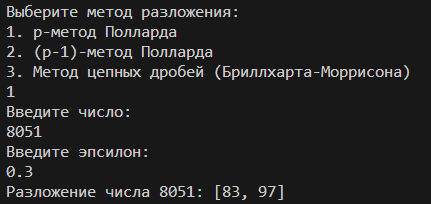
\includegraphics[width=0.8\textwidth]{pic/1.png}
            \caption{Тест первого алгоритма факторизации чисел}
        \end{figure}

        \begin{figure}[H]
            \centering
            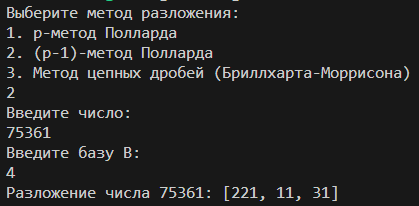
\includegraphics[width=0.8\textwidth]{pic/2.png}
            \caption{Тест второго алгоритма факторизации чисел}
        \end{figure}

        \begin{figure}[H]
            \centering
            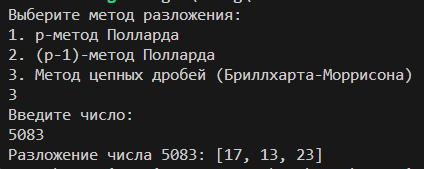
\includegraphics[width=0.8\textwidth]{pic/3.png}
            \caption{Тест третьего алгоритма факторизации чисел}
        \end{figure}

\conclusion

    В данной лабораторной работе были изучены теоретические сведения о методах
    факторизации чисел ($\rho$-метод Полларда, $(\rho-1)$-метод Полларда,
    алгоритм Бриллхарта-Моррисона). На их основе были рассмотрены
    соответствующие алгоритмы. Была произведена оценка сложности созданных
    алгоритмов. Они послужили фундаментом для программной реализации, которая
    впоследствии успешно прошла тестирование, результаты которого были
    прикреплены к отчету вместе с листингом программы, написанной на языке Rust
    с использованием стандартных библиотек языка.

\end{document}
